% MARCO TEÓRICO

\cleardoublepage

\chapter{Marco teórico}

En este capítulo se va a profundizar en la teoría que sustenta la generación de contenidos y dentro de ello, la generación musical. Para que el lector no tenga que dar nada por sentado, se va a hacer un repaso desde la generación del sonido, captación, transformación, codificación y guardado, hasta la aprehensión de conocimiento por parte de un sistema de Inteligencia Artificial y la posterior generación de nuevo conocimiento, completando así el círculo que se dejó abierto en los pasos previos de codificación, donde se tenían datos, hasta llegar transformarlos y obtener información a partir de ellos, para después poder generar nuevas piezas musicales.

\section{Del sonido a los bytes: proceso de captación, transformación y discretización}

\subsection{La naturaleza del Sonido}
El sonido es una onda mecánica que se propaga a través de un medio elástico, como el aire, el agua o un cuerpo sólido. El sonido se genera cuando un objeto vibra, haciendo que las moléculas del medio se agiten alrededor de su posición de reposo. Esto forma perturbaciones en forma de ondas longitudinales. La figura \ref{fig:onda_sonora} muestra un diagrama de cómo se produce este fenómeno y el patrón de perturbación longitudinal que produce.

\begin{figure}[H]
  \centering
  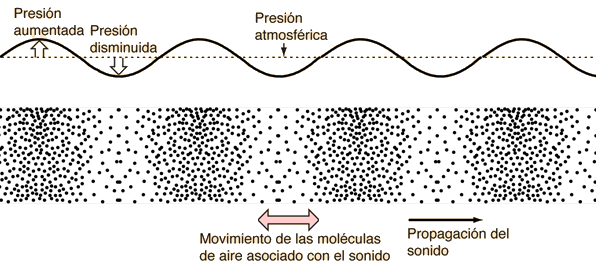
\includegraphics[width=0.9\textwidth]{images/wave.png}
  \caption{Onda sonora.}
  \label{fig:onda_sonora}
\end{figure}

Las propiedades principales del sonido son:

\subsubsection{Frecuencia ($f$)}
Determina el tono de un sonido. Se define como:
\begin{equation}
    f = \frac{1}{T}
\end{equation}
donde $T$ es el período de la onda en segundos. En términos de la velocidad de propagación $v$ y la longitud de onda $\lambda$, la frecuencia también puede expresarse como:
\begin{equation}
    f = \frac{v}{\lambda}
\end{equation}

Se mide en Hertz (Hz). Una mayor frecuencia corresponde a sonidos más agudos, mientras que una menor frecuencia genera sonidos más graves. El oído humano puede detectar frecuencias en el rango de 20 Hz a 20 kHz.

\subsubsection{Amplitud ($A$)}
La amplitud es la máxima elongación de la onda respecto a su posición de equilibrio. Está relacionada con la intensidad del sonido percibido.
\begin{equation}
    I = 10 \log_{10} \left( \frac{P}{P_0} \right)
\end{equation}
donde $P$ es la potencia de la onda sonora y $P_0$ es la potencia de referencia estándar (normalmente $10^{-12}$ W/m$^2$ en aire).

Se mide en decibelios (dB). Los sonidos de mayor amplitud se perciben como más fuertes; por el contrario, los de menor amplitud son más suaves.

\subsubsection{Longitud de onda ($\lambda$)}
La longitud de onda es la distancia entre dos puntos consecutivos en fase (por ejemplo, de cresta a cresta) y está dada por:
\begin{equation}
    \lambda = \frac{v}{f}
\end{equation}

En medios distintos del aire, la longitud de onda varía debido a cambios en la velocidad de propagación. Por ejemplo, en el agua, donde el sonido viaja a aproximadamente 1482 m/s, la misma frecuencia produce una longitud de onda mayor que en el aire.

\subsubsection{Velocidad de propagación ($v$)}
La velocidad del sonido depende del medio a través del cual se propaga y se determina mediante:
\begin{equation}
    v = \sqrt{\frac{B}{\rho}}
\end{equation}
donde $B$ es el módulo de elasticidad del medio y $\rho$ su densidad.

En distintos medios, la velocidad del sonido varía significativamente:
\begin{itemize}
    \item Aire (20$^\circ$C): 343 m/s
    \item Agua: 1482 m/s
    \item Acero: 5960 m/s
\end{itemize}

\subsubsection{Presión sonora ($p$)}
El sonido también puede describirse en términos de presión acústica, relacionada con la intensidad de la onda por:
\begin{equation}
    I = \frac{p^2}{\rho v}
\end{equation}

Esta presión es responsable de cómo percibimos el volumen del sonido. Se mide en Pascales (Pa).

\subsubsection{Intensidad del sonido ($I$)}
La intensidad del sonido mide la cantidad de energía que transporta una onda sonora por unidad de área y se expresa como:
\begin{equation}
    I = \frac{P}{A}
\end{equation}

\subsubsection{Amplitud ($A$) e Intensidad ($I$)}
La amplitud es la máxima elongación de la onda respecto a su posición de equilibrio. Está relacionada con la intensidad del sonido percibido, que se mide en decibeles (dB) y se expresa como:
\begin{equation}
    I = 10 \log_{10} \left( \frac{P}{P_0} \right)
\end{equation}
donde $P$ es la potencia de la onda sonora y $P_0$ es la potencia de referencia estándar (normalmente $10^{-12}$ W/m$^2$ en aire).

Sonidos de mayor amplitud se perciben como más fuertes, mientras que los de menor amplitud son más suaves.

\begin{tcolorbox}[title=Relación entre Amplitud e Intensidad,colback=gray!10, colframe=gray!50, sharp corners=south]
La amplitud representa la variación de presión en el medio por efecto de la onda sonora. La intensidad sonora, en cambio, está relacionada con la percepción subjetiva del volumen. Aunque están correlacionadas, la percepción auditiva del volumen no es lineal respecto a la amplitud. Se rige en una escala logarítmica.\vspace{10pt}

\parbox{\textwidth}{\textbf{Cómo percibe el oído los cambios de amplitud e intensidad}}
El sistema auditivo humano no responde de manera proporcional a los cambios en la amplitud de las ondas sonoras.

Un sonido de doble de amplitud no se percibe como ``el doble de fuerte''. Para que un sonido se perciba ``el doble de fuerte'', su intensidad debe aumentar aproximadamente 10 veces. Cada incremento de 10 dB en intensidad se siente como un sonido aproximadamente el doble de fuerte.

El oído humano es más sensible a ciertos rangos de frecuencia, lo que significa que los cambios de amplitud pueden percibirse de manera distinta según la frecuencia del sonido. Por ejemplo, contando con la misma amplitud, sonidos de 1000 Hz son percibidos con mayor intensidad que sonidos de 100 Hz.\vspace{10pt}

\parbox{\textwidth}{\textbf{Ejemplos de percepción de cambios de amplitud, intensidad y ambos}}
\begin{itemize}
    \item \emph{Cambio de amplitud}: golpear un tambor con más fuerza produce un sonido más fuerte sin cambiar su tonalidad (se mantiene la frecuencia).
    \item \emph{Cambio de intensidad}: Aumentar el volumen de una radio mantiene la misma música pero a un nivel sonoro más alto.
    \item \emph{Cambio de ambos}: un grito, que comienza como un susurro y termina en un grito fuerte, no solo varía en amplitud, sino que también cambia en intensidad progresivamente.
\end{itemize}

Los cambios en amplitud pueden detectarse más fácilmente en sonidos de corta duración o con transiciones bruscas, como golpes de tambor o explosiones, mientras que cambios en intensidad pueden ser más notorios en sonidos sostenidos.

Este comportamiento explica por qué los ajustes de volumen en dispositivos de audio son exponenciales en lugar de lineales.
\end{tcolorbox}

\subsubsection{Timbre}
El timbre es la característica del sonido que permite diferenciar dos sonidos de igual frecuencia y amplitud, que son generados por fuentes diferentes. Está determinado por la composición espectral de la onda sonora, es decir, la combinación de frecuencias fundamentales y armónicas presentes en el sonido. Matemáticamente, se representa como la suma de ondas sinusoidales:
\begin{equation}
    S(t) = \sum_{i=1}^{n}n A_i \cos(\omega_i t)
\end{equation}
donde cada término representa un armónico con su propia amplitud y frecuencia.

El timbre es un elemento clave y central en la música y en la percepción del habla, pues es la propiedad que hace único el sonido de cada instrumento o la voz de una persona.

\subsection{Captura del Sonido}
Para digitalizar el sonido, primero es necesario \textbf{capturarlo} utilizando un transductor, que convierte la energía acústica, en forma de vibraciones en el medio, en una señal eléctrica. Estos dispositivos pueden ser, por ejemplo:

\begin{itemize}
    \item \textbf{Micrófonos}: capturan ondas de sonido y las convierten en señales eléctricas.
    \item \textbf{Pastillas de guitarra}: detectan vibraciones de las cuerdas y las transforman en corriente eléctrica.
    \item \textbf{Sensores piezoeléctricos}: utilizados en pianos eléctricos y otros instrumentos electrónicos.
\end{itemize}

La señal eléctrica obtenida sigue siendo analógica y debe ser convertida en una representación digital mediante un convertidor \emph{Analógico-Digital \textbf{(A/D)}}.

\subsection{Muestreo}
El sonido en su forma natural es una \textbf{onda analógica}, lo que significa que tiene una variabilidad infinita en el tiempo y la amplitud. Sin embargo, las computadoras y dispositivos digitales solo pueden manejar información en forma de números discretos. Para convertir una señal analógica en digital, es necesario \textbf{tomar muestras} de la amplitud del sonido en distintos instantes de tiempo.

Este proceso se asemeja a tomar fotografías de una escena en movimiento a una tasa constante: cuanto mayor sea la cantidad de fotos por segundo (tasa de muestreo), más suave y precisa será la representación de la escena.

\section{Frecuencia de Muestreo}

La \textbf{frecuencia de muestreo} determina cuántas veces por segundo se toma una muestra de la señal de audio. Se mide en \textbf{Hertz (Hz)} y sigue el \textbf{Teorema de Nyquist-Shannon}, que establece que la frecuencia de muestreo debe ser al menos \textbf{el doble de la frecuencia más alta contenida en la señal original}:

\begin{equation}
    f_s \geq 2 f_{max}
\end{equation}

donde:
\begin{itemize}
    \item $f_s$ es la frecuencia de muestreo.
    \item $f_{max}$ es la frecuencia más alta en la señal de entrada.
\end{itemize}

Si este criterio no se cumple, se produce \textbf{aliasing}, un efecto en el que las frecuencias más altas se distorsionan y terminan representándose incorrectamente en el audio digital.

Ejemplo de \textbf{frecuencias de muestreo comunes}:
\begin{itemize}
    \item \textbf{44.1 kHz}: usado para codificar sonido en CD de audio. Permite captar frecuencias hasta \textbf{22.05 kHz}.
    \item \textbf{48 kHz}: utilizado en audio para video y grabaciones estándar.
    \item \textbf{96-192 kHz}: aplicado en grabaciones de alta fidelidad y producción de estudio.
\end{itemize}

\subsection{Cuantización: Representación Numérica de las Muestras}

Cada muestra tomada en el proceso de muestreo debe convertirse en un valor numérico finito. Este proceso se llama \textbf{cuantización}, y su precisión depende de la \textbf{profundidad de bits}.

Ejemplos de resoluciones comunes:
\begin{itemize}
    \item \textbf{8 bits} – 256 niveles posibles (baja calidad, usada en telefonía).
    \item \textbf{16 bits} – 65,536 niveles (calidad estándar de CD).
    \item \textbf{24 bits} – 16,777,216 niveles (grabaciones profesionales).
\end{itemize}

Cuanto mayor es la profundidad de bits, menor es el \textbf{ruido de cuantización}, que es la diferencia entre la señal original y su versión cuantizada.

\subsection{Alias y pérdida de información}

Si la frecuencia de muestreo es demasiado baja, se produce un fenómeno llamado \textbf{aliasing}, en el cual las frecuencias más altas aparecen distorsionadas y se confunden con frecuencias más bajas.

Para evitar esto, se utilizan \textbf{filtros antialiasing} antes de la digitalización, que eliminan las frecuencias superiores a la mitad de la frecuencia de muestreo.

Ejemplo:
\begin{itemize}
    \item Si se digitaliza una señal con \textbf{una frecuencia de muestreo de 20 kHz}, pero la señal contiene componentes de hasta \textbf{30 kHz}, estas frecuencias más altas se distorsionarán.
\end{itemize}

\subsection{Aplicaciones del Muestreo}

\begin{table}[H]
    \centering
    \caption{Frecuencia de muestreo y profundidad de bits según la aplicación.}
    \begin{tabular}{|l|c|c|}
        \hline
        \textbf{Aplicación} & \textbf{Frecuencia de Muestreo} & \textbf{Profundidad de Bits} \\
        \hline
        \textbf{Telefonía digital} & 8 kHz & 8 bits \\
        \textbf{Radio FM} & 32 kHz & 12 bits \\
        \textbf{CD de audio} & 44.1 kHz & 16 bits \\
        \textbf{Grabaciones de estudio} & 96-192 kHz & 24 bits \\
        \hline
    \end{tabular}
    \label{tabla:frecuencia_muestreo}
\end{table}

La tabla \emph{Frecuencia de muestreo y profundidad de bits según la aplicación} \ref{tabla:frecuencia_muestreo} muestra una tabla comparativa de usos, frecuencias de muestreo y profundidad (o anchura) de bits utilizados en su representación digital.

\subsection{Percepción Auditiva y Frecuencia de Muestreo}

El oído humano tiene una respuesta no lineal a las frecuencias y la amplitud del sonido. Aunque el rango audible se encuentra entre \textbf{20 Hz y 20 kHz}, la sensibilidad es mayor en el rango de \textbf{1 kHz a 5 kHz}, donde se encuentra la mayor parte del contenido del habla.

\subsection{Reconstrucción del Sonido Digitalizado}

Después de la digitalización, el sonido debe convertirse nuevamente en una señal analógica para ser escuchado. Esto se realiza mediante un \textbf{convertidor digital-analógico (DAC)}, que:
\begin{enumerate}
    \item \textbf{Interpola} los valores entre muestras para suavizar la transición.
    \item \textbf{Usa un filtro de reconstrucción} para eliminar artefactos digitales.
    \item \textbf{Produce una señal analógica continua} para su reproducción.
\end{enumerate}

\section{MP3: un formato reducido}

El formato MP3 marcó un antes y un después en la digitalización del sonido. Fue el vehículo que revolucionó el consumo de música, popularizando el formato de audio digital, combinando eficiencia de compresión y facilidad de reproducción con \emph{códecs}. Dio nombre a pequeños aparatos que durante la primera década de los años 2000 inundaron bolsillos, dando la posibilidad de tener varios discos de música en el mismo espacio que un llavero. Fue, sin saberlo, el vehículo que abrió la puerta a la piratería y a la compartición ilícita de ficheros.

\subsection{Codificación y formatos de audio}

Una vez que la señal de audio ha sido muestreada y cuantificada, es necesario almacenarla en un formato digital adecuado. Para ello, los datos obtenidos son organizados en estructuras llamadas \textbf{códecs} (codificador/decodificador), que definen cómo se comprimen y guardan los archivos de audio.

Los formatos de audio digital pueden dividirse en tres grandes categorías:

\begin{enumerate}
    \item \textbf{Formatos sin compresión}: Guardan la señal tal cual fue capturada, sin ninguna reducción de datos. Ejemplos:
    \begin{itemize}
        \item \textbf{PCM} (Pulse Code Modulation): base de todos los formatos sin compresión.
        \item \textbf{WAV} (Waveform Audio File Format): utilizado en entornos profesionales por su fidelidad.
        \item \textbf{AIFF} (Audio Interchange File Format): equivalente de WAV para sistemas Mac.
    \end{itemize}
    
    \item \textbf{Formatos comprimidos sin pérdida}: Reducen el tamaño del archivo sin eliminar información del sonido original. Ejemplos:
    \begin{itemize}
        \item \textbf{FLAC} (Free Lossless Audio Codec): muy popular en audiófilos y distribución digital de alta calidad.
        \item \textbf{ALAC} (Apple Lossless Audio Codec): alternativa de Apple al FLAC.
        \item \textbf{APE} (Monkey’s Audio): menos común, pero con tasas de compresión más altas.
    \end{itemize}

    \item \textbf{Formatos comprimidos con pérdida}: fruto de algoritmos de compresión perceptual, el tamaño ha sido reducido al máximo exponente posible, eliminando partes de la señal consideradas inaudibles. Ejemplos:
    \begin{itemize}
        \item \textbf{MP3} (MPEG-1 Audio Layer III): el más famoso y extendido.
        \item \textbf{AAC} (Advanced Audio Codec): formato utilizado en iTunes, YouTube y Spotify, con mejor calidad que MP3 al mismo nivel de \emph{bitrate}.
        \item \textbf{OGG Vorbis}: alternativa libre con mejor calidad que MP3, usada en videojuegos y streaming.
    \end{itemize}
\end{enumerate}

\section{Bitrate: Definición y su impacto en la calidad del MP3}

Antes de continuar, es necesario aclarar un concepto clave en la codificación eficiente y correcta de música en MP3.

\subsection{¿Qué es el bitrate?}
El \textbf{bitrate} es la tasa cantidad de datos en un segundo del fichero de audio. Se mide en \textbf{kilobits por segundo (kbps)} y determina la calidad y el tamño del fichero de la siguiente manera:
\begin{itemize}
    \item \textbf{Bitrate alto}: mayor calidad de audio y ficheros de mayor tamaño.
    \item \textbf{Bitrate bajo}: menor calidad y archivos más pequeños.
\end{itemize}

\subsection{Bitrates máscomunes en MP3 y su calidad percibida}
El MP3 permite codificar audio en diferentes bitrates, cada uno con una calidad de sonido distinta.

\begin{table}[H]
    \centering
    \caption{Comparación de bitrates y calidad de sonido en el formato MP3.}
    \resizebox{\textwidth}{!}{%
    \begin{tabular}{|c|l|l|}
        \hline
        \textbf{Bitrate (kbps)} & \textbf{Calidad percibida} & \textbf{Uso típico} \\
        \hline
        320 kbps  & Casi idéntico al original & Audio de alta calidad, producción musical \\
        256 kbps  & Excelente calidad, mínima pérdida & Descargas de alta fidelidad, iTunes \\
        192 kbps  & Buena calidad, ligera pérdida & Streaming de alta calidad, radio online \\
        160 kbps  & Calidad aceptable & Spotify estándar, radio digital \\
        128 kbps  & Pérdida de detalles en frecuencias altas & Antiguas descargas MP3, radio FM \\
        96 kbps   & Pérdida notable, sonido más plano & Podcasts, audiolibros \\
        64 kbps   & Baja calidad, sonido metálico & Streaming de voz, radio de baja calidad \\
        32 kbps o menos & Calidad muy pobre, muchas pérdidas & Uso extremo en redes con bajo ancho de banda \\
        \hline
    \end{tabular}
    }
    \label{tab:bitrates}
\end{table}

En la tabla \emph{Comparación de bitrates y calidad de sonido en el formato MP3}\ref{tab:bitrates} se recogen los valores más comunes.

\subsection{¿Cuál es un bitrate adecuado?}
El bitrate óptimo depende del uso específico y del balance entre calidad y tamaño del archivo:

\begin{itemize}
    \item Para \textbf{escuchar música con buena calidad}, un bitrate de 192 kbps es un buen punto intermedio.
    \item Para \textbf{calidad similar a la de un CD}, se recomienda 320 kbps en formato MP3.
    \item Para \textbf{streaming}, los servicios más utilizados emplean tasas variables:
    \begin{itemize}
        \item \textbf{Spotify}: 96 kbps (básico), 160 kbps (normal), 320 kbps (premium).
        \item \textbf{YouTube Music}: Dependiendo de la conexión, varía entre 48 kbps y 256 kbps en AAC.
    \end{itemize}
\end{itemize}

\subsection{Efectos de un bitrate bajo en la calidad del audio}
La compresión MP3 reduce el tamaño del archivo eliminando datos considerados menos perceptibles para el oído humano. Sin embargo, si el bitrate es demasiado bajo, ocurre que:

\begin{enumerate}
    \item Se eliminan demasiadas \textbf{frecuencias altas}, reduciendo la claridad del sonido.
    \item Aparecen \textbf{artefactos de compresión} (ruidos metálicos, eco, distorsión).
    \item Se pierde \textbf{profundidad y riqueza sonora}, dando una sensación de audio plano.
\end{enumerate}

Bitrates menores de 128 kbps producen diferencias, con el audio original, audibles en reproductores más básicos, afectando la experiencia de escucha.

\subsubsection{MP3: Compresión perceptual y revolución digital}

El formato \textbf{MP3} (MPEG-1 Audio Layer III) se convirtió en el estándar de facto para la música digital gracias a su gran capacidad de reducción del tamaño de los archivos, sin una pérdida de calidad perceptible en \emph{bitrates} determinados.

\subsubsection{Ventajas del MP3}
\begin{itemize}
    \item \textbf{Alta eficiencia en almacenamiento}: Un archivo MP3 puede ser hasta \textbf{10 veces más pequeño} que su equivalente en WAV sin comprimir.
    \item \textbf{Compatibilidad universal}: Es reproducible en prácticamente cualquier dispositivo, desde teléfonos móviles hasta sistemas de sonido profesionales.
    \item \textbf{Facilidad de distribución}: Su tamaño reducido lo hizo ideal para la difusión de música en Internet, dando lugar a plataformas como Napster en los 2000 y posteriormente al auge del streaming.
\end{itemize}

\subsubsection{Desventajas del MP3}
\begin{itemize}
    \item \textbf{Pérdida de calidad}: A bitrates bajos (como 128 kbps), pueden aparecer artefactos sonoros y pérdida de claridad en frecuencias altas.
    \item \textbf{Formatos más eficientes lo han superado}: Actualmente, códecs como \textbf{AAC, Opus y FLAC} han reemplazado al MP3 en muchas plataformas de streaming y almacenamiento de alta calidad.
\end{itemize}

%\subsection{Impacto del MP3 en la industria musical}
%El MP3 cambió para siempre la forma en que se consume la música. Su aparición permitió la popularización de la música digital, pero también trajo consigo desafíos para la industria:

%\begin{itemize}
%    \item \textbf{Explosión de la piratería}: La facilidad de compartir archivos MP3 a través de Internet llevó a la creación de plataformas como \textbf{Napster}, lo que causó una crisis en la industria discográfica.
%    \item \textbf{Cambio en los modelos de negocio}: Las disqueras tuvieron que adaptarse al formato digital, dando paso a servicios como \textbf{iTunes, Spotify y Apple Music}.
%    \item \textbf{Transición hacia el streaming}: Con el aumento de la velocidad de Internet, el almacenamiento local de archivos MP3 ha disminuido en favor de la transmisión en tiempo real.
%\end{itemize}

\section{De los datos a la información}

La información no es más que datos con significado. Partiendo de esta idea, los datos se podrían enunciar como la unidad mínima que compone la información, una vez estos son interpretados.

Para ello, es necesario tratarlos, guardarlos, manejarlos correctamente, transformarlos... en esencia, adecuarlos para extraer toda la información posible.


\subsection{Tratamiento de los datos}

Para el entrenamiento de los modelos basados en Inteligencia Artificial que se plantearán para cumplir los objetivos, se van a utilizar 3 extensos datasets, cuyo tamaño y diversidad de géneros musicales contenidos abran posibilidad de poder obtener una herramienta que tenga un desempeño a la altura de lo que se podría esperar.

Asi pues, los 3 datasets propuestos son:

\subsubsection{FMA (Free Music Archive) Dataset}

Con un tamaño de más de 100,000 pistas y 160 géneros, se trata de un \emph{dataset} enorme, que cuenta con piezas representativas de cada género. Está respaldado por un repositorio \href{https://github.com/mdeff/fma}{GitHub} que además provee unos \emph{scripts} con ejemplos y algoritmos en \emph{Python}, que extraen información sobre estructura, contenido, organización, etc., del conjunto de datos.

Todas las pistas se encuentran en formato \emph{MP3} (44.1 kHz, 128-320 kbps). Existen tres variantes en cuanto al tamaño del conjunto de datos:

\begin{itemize}
    \item \textbf{FMA Small:} 8,000 pistas, 8 géneros, aproximadamente 1GB.
    \item \textbf{FMA Medium:} 25,000 pistas, 16 géneros, aproximadamente 10GB.
    \item \textbf{FMA Large:} 106,000 pistas, 161 géneros, aproximadamente 100GB. \textbf{(Esta ha sido la variante utilizada).}
\end{itemize}

Se incluyen metadatos como título, artista, álbum, y etiquetas de género. Los géneros musicales están repartidos en niveles de manera jerárquica, siendo los géneros \emph{parent} de primer orden los siguientes:

\begin{multicols}{4}
\begin{itemize}
    \item Blues
    \item Classical
    \item Country
    \item Disco
    \item Hip-Hop
    \item Jazz
    \item Metal
    \item Pop
    \item Reggae
    \item Rock
\end{itemize}
\end{multicols}

\subsubsection{Million Song Dataset}

Se trata de un \emph{dataset vivo}. De base, cuenta con 1500 ficheros en formato \emph{MP3}, distribuidos en 15 categorías de género. Sin embargo, \href{https://www.kaggle.com/datasets/undefinenull/million-song-dataset-spotify-lastfm}{este conjunto de datos} puede hacerse tan grande como se necesite, pues viene acompado de unos ficheros \emph{Python} que realizan una integración con servicios como Spotify y Last.fm. Además de eso, la sincronización con estos dos servicios brinda acceso a metadatos sobre popularidad, características del sonido y etiquetas de géneros.

Así pues, se podría decir que este \emph{dataset} brinda la posibilidad de tener ``toda'' la música de la red disponible para trabajar con ella.

Los géneros de los que se dispone son:
\begin{multicols}{4}
\begin{itemize}
    \item Electronic
    \item Rock
    \item Pop
    \item Folk
    \item Jazz
    \item Blues
    \item Country
    \item Reggae
    \item Latin
    \item R\&B
    \item World
    \item Rap
    \item Punk
    \item New Age
    \item Metal
\end{itemize}
\end{multicols}

\subsubsection{MTG-Jamendo Dataset}

Este \emph{dataset} cuenta con más de 50,000 pistas y 190 géneros, en ficheros \emph{MP3} de 320 kbps . Enorme donde los haya, esta librería fue desarrollada para tareas de etiquetado automático de música. Contiene un conjunto de etiquetas entre las que se encuentran: géneros musicales, instrumentos, emociones y temas. Viene respaldado por un repositorio \href{https://github.com/MTG/mtg-jamendo-dataset}{GitHub} que provee de scripts para su descarga y manejo, así como información sobre su contenido e información estadística.

Los géneros que se pueden encontrar, entre otros, son:
\begin{multicols}{4}
\begin{itemize}
    \item Electronic
    \item Rock
    \item Pop
    \item Folk
    \item Jazz
    \item Hip-Hop
    \item Classical
    \item Reggae
    \item Ska
    \item Swing
    \item Fusion
    \item Easy Listening
    \item Opera
    \item Gospel
    \item Holiday
    \item Comedy
    \item Spoken Word
    \item Podcast
    \item Sound Effects
\end{itemize}
\end{multicols}

Dentro de las modalidades de \emph{dataset} que provee este repositorio, se ha elegido \emph{autotagging\_moodtheme}, que provee ficheros de 30 segundos de duración con etiqueta de género, entre otras.

%python3 scripts/download/download.py --dataset autotagging_moodtheme --type audio  /media/luke/32B841C3B8418677/VIU\ dataset\ mtg/ --unpack

%\subsubsection{Tabla comparativa de tramos entre datasets}
%\begin{table}[h]
\caption{Resumen comparativo de los datasets utilizados}
\centering
\begin{tabular}{|l|l|l|l|}
\hline
\textbf{Dataset} & \textbf{Formato} & \textbf{Volumen} \\ \hline
FMA & MP3 & Hasta 106,000 pistas \\ \hline
Million Song Dataset & MP3 & 1500 (ampliable bajo integración)  \\ \hline
MTG-Jamendo & MP3 & 55,000 pistas \\ \hline
\end{tabular}
\end{table}

\subsection{Aprendiendo sobre géneros musicales}

Según la \emph{Real Academia Española} (RAE), \emph{aprender} se define como ``adquirir el conocimiento de algo por medio del estudio o de la experiencia''\citep{rae_aprender}. Entiéndase el estudio como ese ejercicio mental para llegar a esos conocimientos. Pero el estudio, planteado así, es algo inherente al humano. Ni siquiera los animales tendrían la capacidad de estudiar. Cuanto menos, una máquina.

Por lo tanto, la única manera que tendría una ordenador de aprender sería \emph{adquirir experiencia}. De la misma manera que un ratón de laboratorio, durante múltiples experimentos, puede ir recordando, \emph{amoldando} sus \emph{recuerdos} con los eventos que van aconteciendo, en el aprendizaje profundo o \emph{Deep Learning}, la estructura de red neuronal que va haciéndose eco de esos cambios que se van sucediendo, se convierte en una herramienta poderosísima para el análisis y clasificación de datos complejos, incluida la música y las pautas que la describen. 

Este tipo de aprendizaje permite a los modelos identificar patrones ocultos y aprender características específicas de distintos géneros, de la misma manera que lo haría un oyente que nunca ha escuchado música antes y que carece de conocimientos musicales: oyendo \emph{miles de veces cientos de canciones distintas} o lo que es lo mismo: explorando grandes conjuntos de datos \emph{etiquetados} (de alguna manera).

Una de las formas de realizar este análisis es el uso de redes neuronales convolucionales (\emph{Convolutional Neural Networks}, CNN) junto con algún mecanismo que implemente \emph{memoria recurrente} para dicha red, como por ejemplo los (\emph{Long Short-Term Memory}, LSTM). Basadas en el reconocimiento de imágnenes, este tipo de redes han supuesto un antes y un después en la visión (y aprehensión visual) por computadora. Una de las características más llamativas de este tipo de redes es la arquitectura \emph{hardware} sobre la que se suele apoyar: usa la \emph{GPU} en vez del procesador central de la máquina, dada la naturaleza matricial de la representación de los datos en imágenes.

Pero si la música es sonido, ¿cómo puede una \emph{CNN} analizar audio?: extrayendo la representación espectral del sonido o espectrograma y analizando una imagen del mismo; a su vez, las LSTM manejarían secuencias temporales de datos musicales, permitiendo modelar la continuidad y dependencia entre las notas.

En este trabajo se van a abordar dos maneras equivalente de hacer esto, teniendo en cuenta las últimas tendencias en Inteligencia Artificial.

\subsection{Variational Autoencoders (VAE)}

Los \textbf{Autoencoders} son redes neuronales diseñadas para aprender una representación codificada y ``comprimida'' de los datos de entrada, con el fin de ser reconstruidos cometiendo el menor error posible. Esto es, en definitiva, \textbf{aprender las características esenciales de los datos} y cofificarlas \textbf{en un espacio de menor dimensión.}

La figura \ref{fig:vae} ilustra cómo sería la arquitectura base.

\begin{figure}[H]
  \centering
  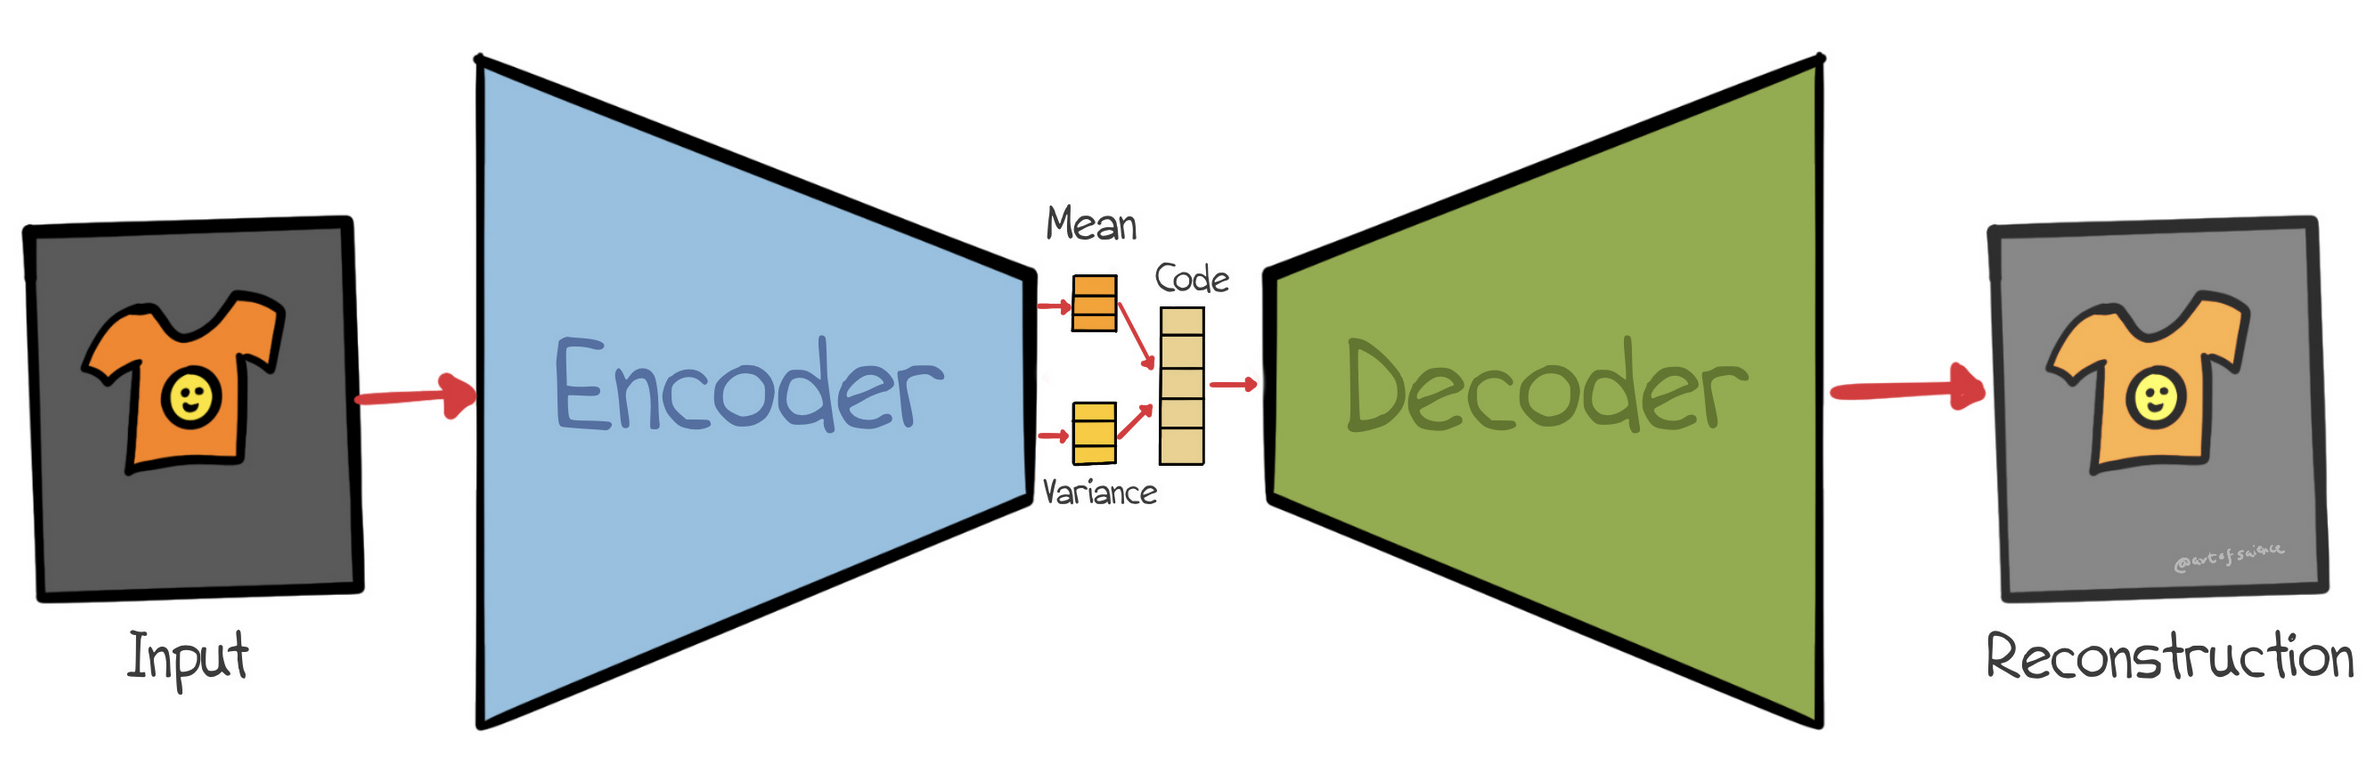
\includegraphics[width=0.9\textwidth]{images/vae.png}
  \caption{Variational Autoencoder.}
  \label{fig:vae}
\end{figure}

Ésta se compone de:

\begin{enumerate}
    \item \textbf{Codificador (Encoder)}: transforma la entrada original en una representación comprimida de menor dimensión.
    \item \textbf{Espacio latente}: representación interna de los datos. Albergará las caractarísticas principales de los datos usando una menor dimensión. Es el alma del autoencoder.
    \item \textbf{Decodificador (Decoder)}: reconstruye la entrada original (o lo intenta) a partir de la representación de los datos en el espacio latente.
\end{enumerate}


Haciendo un símil, al igual que cuando una persona cuenta un chiste y otra lo escucha para poder volverlo a contar, el receptor no retiene todos los detalles de la historia, sólo necesita recordar \textbf{la esencia de la gracia}, para volver a \emph{contar el chiste} de nuevo.

El entrenamiento de estas redes busca minimizar una \textbf{función de pérdida de reconstrucción}, que marcará la la diferencia entre la entrada original y la reconstrucción: entrada y salida del autoencoder; se puede utilizar, por ejemplo, el \emph{Mean Square Error} (MSE):

\begin{equation}
    L(x, \hat{x}) = \| x - \hat{x} \|^2
\end{equation}

Donde \( x \) es la entrada original y \( \hat{x} \) la salida reconstruida por el decodificador.

Uno de los problemas que presenta este modelo es que el espacio latente no está ordenado. Es decir: no se atiene a unas normas o reglas en las que la información esté estructurada o cuya ordenación tenga algún significado. Simplemente se han ido almacenando datos y serán utilizados para la fase de decodificación (generación).

Además de esto, disponen de una \emph{baja variabilidad generativa}, pues están diseñados para saber \emph{reproducir la entrada} solamente. Esto también llevará a un sobreajuste de la red.

Para paliar estas limitaciones, aparece la idea de \textbf{Autoencoders Variacionales (VAE)}. Enfocando todos los esfuerzos en dar un orden al espacio latente, en vez de mapear una entrada a un punto específico, los VAE introducen un enfoque probabilístico en dicho espacio, mapeando cada entrada a una \textbf{distribución probabilística \textbf{multivarinate}} en el espacio latente, ofreciendo una mayor variabilidad y capacidad generativa.

Estos nuevos y más sofisticados  autoencoders,\textbf{VAE}, dada su representación de datos en el espacio latente de manera probabilística, representan una herramienta muy útil en la captura y comprensión de características en datos complejos, pues no sólo ``comprimen'' la información, sino que son capaces de capturar estructuras inherentes y distribuciones subyacentes en el espacio de datos (relaciones que en principio no se conocían entre los datos).

De manera análoga, las tres fases de funcionamiento de este nuevo modelo son:

\begin{enumerate}
    \item \textbf{Codificación probabilística}: se asigna cada entrada a una distribución Gaussiana en el espacio latente.
    \item \textbf{Muestreo del espacio latente}: el muestreo desde esta distribución permite la generación de múltiples versiones ``cercanas'' al dato original.
    \item \textbf{Decodificación estocástica}: se reconstruyen las características del dato de entrada a partir de muestras del espacio latente.
\end{enumerate}

Una vez visto esto, la pregunta es: ¿cómo entonces hará un VAE para codificar ficheros \emph{MP3}?

\subsubsection{Procesamiento previo de los datos: de MP3 a números}
\label{proc_mp3}
Los archivos \textbf{MP3} necesitarán un preprocesado para convertir la señal de audio en un formato adecuado para que el VAE, modelo matemático y computable, pueda trabajar con ellos.

El camino a seguir desde el fichero de audio hasta convertirse en datos en el espacio latente conlleva las siguientes fases:

\begin{enumerate}
    \item \textbf{De música en \emph{MP3} a números} \\
    El primer paso es \emph{decodificar el archivo MP3} y convertir la señal de audio a un \emph{array} de valores numéricos que represente el sonido a lo largo del tiempo. Para reducir la dimensionalidad total de la muestra y poderla manejar en piezas más pequeñas, se aplican técnicas de ventana deslizante y la extracción del espectrograma de cada fragmento del archivo, utilizando la Transformada de Fourier de Ventana Corta (STFT):
    \[
        X(t, f) = \sum_{n=0}^{N-1} x(n)w(n-t)e^{-j2\pi fn/N},
    \]
    donde $X(t, f)$ representa el espectrograma del fragmento de audio, $x(n)$ es la señal de entrada, y $w(n)$ es una ventana de análisis.

    \begin{figure}[H]
      \centering
      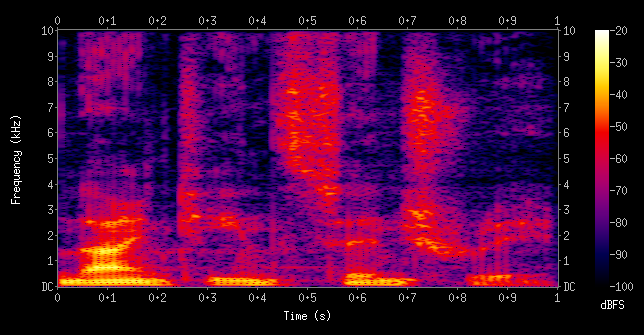
\includegraphics[width=0.85\textwidth]{images/espectrograma.png}
      \caption{Espectrograma}
      \label{fig:espectrograma}
    \end{figure}

    \item \textbf{Representación Espectral (Espectrograma)} \\
    El resultado del STFT es un \emph{espectrograma}, como el que se ve en la figura \ref{fig:espectrograma}, el cual muestra cómo cambia la energía de las distintas frecuencias a lo largo del tiempo. Este espectrograma puede interpretarse como una \emph{imagen} (tratable con una \emph{CNN} tal y como se ha descrito anteriomente), donde las filas representan las frecuencias y las columnas el tiempo.

    \item \textbf{Normalización y Entrada al VAE} \\
    El espectrograma se normaliza para que sus valores estén en un rango definido y se pasa como entrada al VAE. El \emph{codificador} del VAE ``aprenderá'' a comprimir y guardar esta representación en el \emph{espacio latente probabilístico}, asignando cada dato a una distribución Gaussiana multivariante.

    \item \textbf{Representación Latente} \\
    La representación latente captura las \emph{características principales} de la señal de audio: tono, textura del sonido, dinámica temporal... en un espacio mucho más reducido y estructurado, donde será posible \emph{muestrear y obtener nuevas variaciones del sonido}.
\end{enumerate}

Este tipo de autoencoders también podrían utilizarse para:
\begin{itemize}
    \item \textbf{Interpolación de Estilos}: los VAE pueden \emph{combinar estilos musicales distintos}, capturando las transiciones entre ellos y generando nuevos híbridos.
    \item \textbf{Personalización de Características}: permiten modificar atributos específicos, como el tempo, la armonía o la instrumentación, adaptando una pieza musical a las preferencias del usuario.
    \item \textbf{Captura de Coherencia Temporal}: en combinación con redes recurrentes, los VAE mejoran la continuidad temporal de secuencias complejas.
\end{itemize}

\subsection{GANs - Transformers}

Se propone al lector repasar el concepto de \href{https://es.wikipedia.org/wiki/Prueba_de_Turing}{Test de Turing}. Como si de pasar uno de estos test se tratara, existe un modelo de tipo generativo, es decir, diseñado para crear contenido nuevo, que se basa en la \emph{dialéctica} entre sus dos componentes, en la que una de ellas intentará hacer creer a la otra, de ahí la analogía con el test anteriomente citado, que lo que está ``viendo'' no se trata de contenido generado, sino de contenido original.

Las \textbf{GANs (Generative Adversarial Networks)} son unos modelos basados en redes neuronales, diseñados para aprender las características de un conjunto de datos a través de un proceso competitivo, adversarial, entre dos redes: \textit{generador} y \textit{discriminador}. Su capacidad para modelar distribuciones complejas las convierte en herramientas poderosas para captar patrones y relaciones latentes.

\begin{figure}[H]
  \centering
  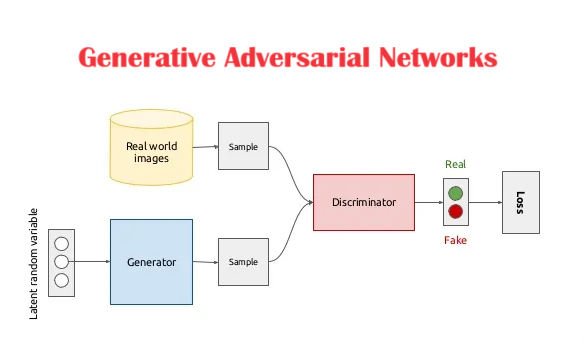
\includegraphics[width=0.8\textwidth]{images/gan.png}
  \caption{GANs (Generative Adversarial Networks)}
  \label{fig:gan}
\end{figure}

La figura \ref{fig:gan} muestra la estructura interna básica de este tipo de modelos, los cuáles se componen de dos elementos básicos:

\begin{itemize}
    \item \textbf{Discriminador (D):} tiene como cometido diferenciar entre datos reales y generados.
    \item \textbf{Generador (G):} su objetivo es generar datos que sean indistinguibles de los datos reales.
\end{itemize}

El entrenamiento de estas dos redes es muy distinto:
\begin{enumerate}
    \item Se entrena el discriminador a parte, con datos reales, los cuáles será capaz de reconocer con un error mínimo.
    \item El generador se entrena produciendo datos a partir de ruido aleatorio. Parte de de una red en principio sin entrenar, que irá variando sus pesos internos, con la diferencia que el discriminador devuelva de comparar (con respecto a la realidad que él sí conoce, dada por la \emph{función de pérdida}) entre cada muestra generada y los datos reales. De esta manera, el discriminador irá haciendo de ``crítico'' en la evaluación de la generación, hasta que el generador consiga engañarlo.
\end{enumerate}

\subsubsection{Transformers y memoria}

Los \textbf{Transformers} son un modelo de Inteligencia Artificial que han revolucionado el campo del aprendizaje secuencial, gracias a su mecanismo de \textit{autoatención}, son capaces de capturar relaciones entre las posiciones de la secuencia de manera paralela, pudiendo así aprender relaciones complejas, en el tiempo y entrenar modelos de mayor tamaño y más eficaces, en menos tiempo. La capacidad para capturar dependencias a largo plazo es lo que las hace tan distintas y valiosas, postulándose como idóneas para la aprehensión de características en \textbf{secuencias de datos (temporales) como texto y audio}.

Introducido por \textbf{Vaswani et al. (2017)} en el artículo \textit{Attention is All You Need}, los Transformers han revolucionando el procesamiento de lenguaje natural (NLP), la visión por computadora, música y generación de texto.

\begin{figure}[H]
  \centering
  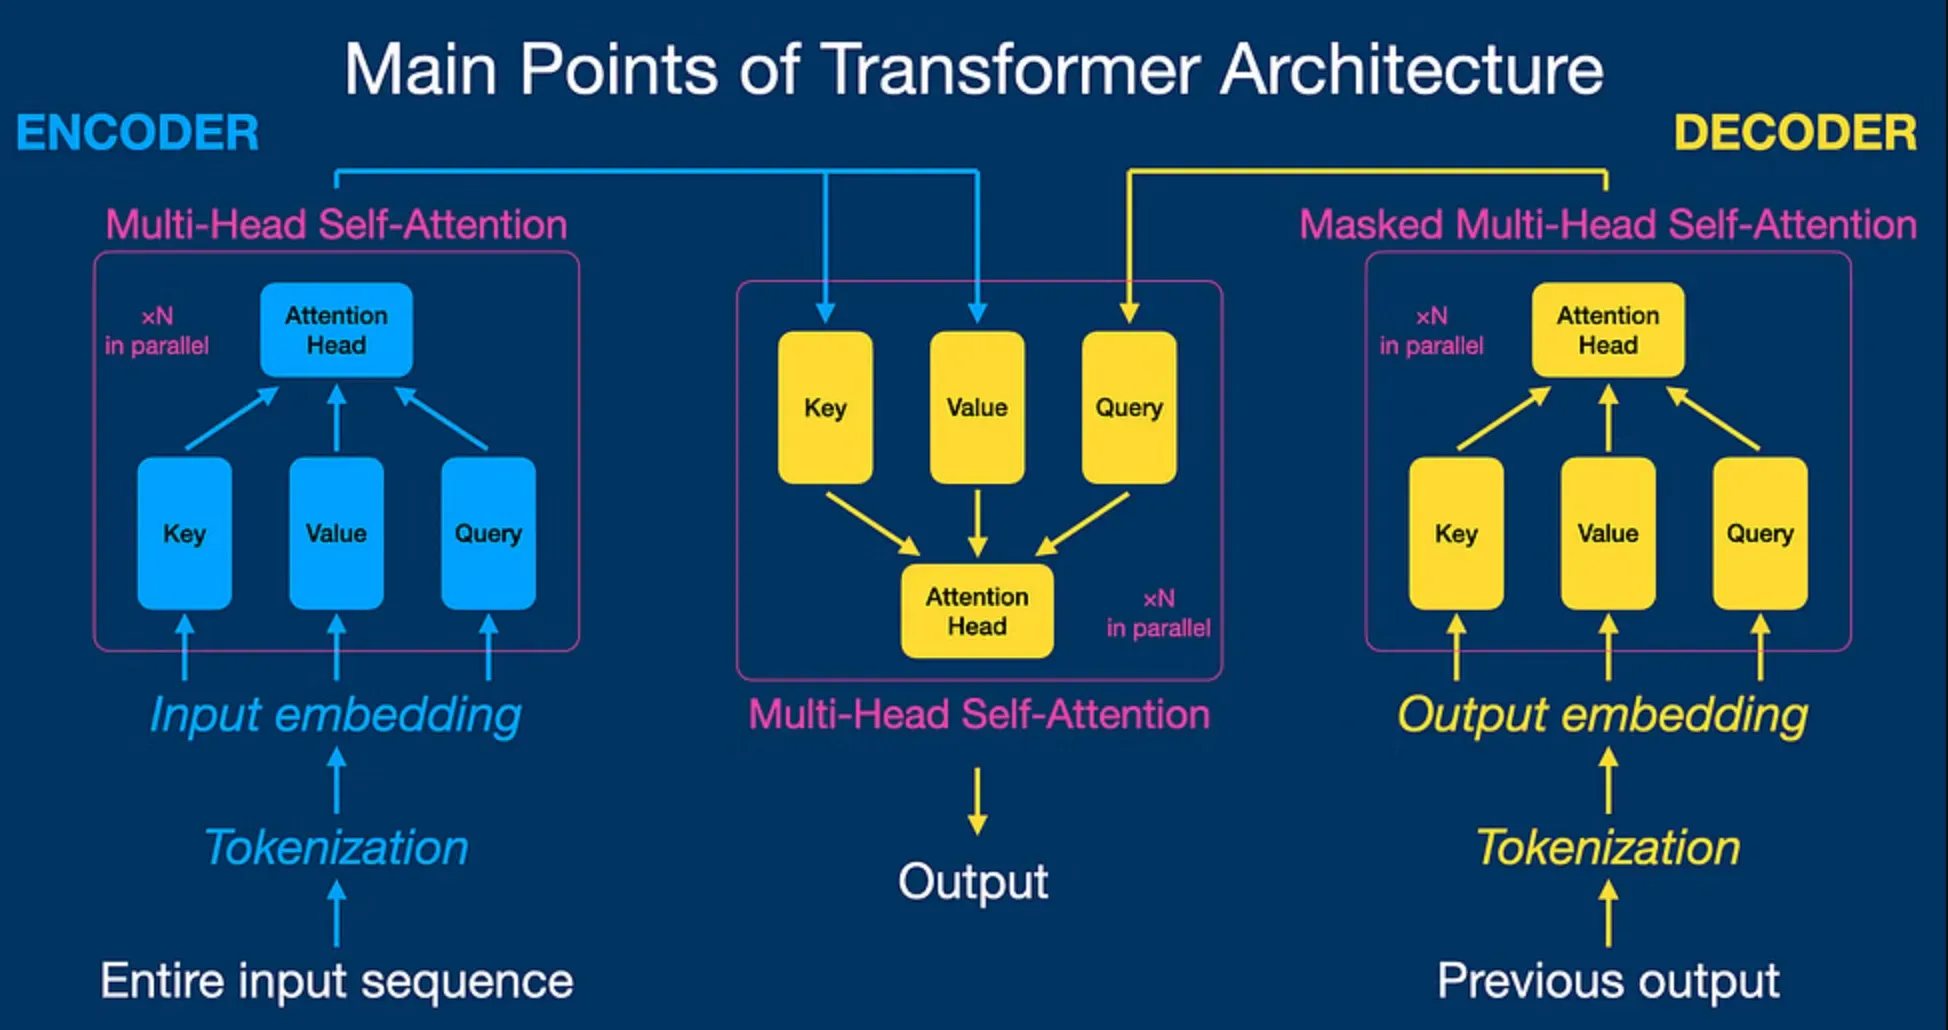
\includegraphics[width=1\textwidth]{images/transformer.png}
  \caption{Transformer Architecture}
  \label{fig:transformer}
\end{figure}

Como queda representado en la figura \ref{fig:transformer}, la arquitectura Transformer consta de \textbf{dos bloques principales}: el \textit{codificador (encoder)} y el \textit{decodificador (decoder)}. Estos trabajan en conjunto para convertir una secuencia de entrada en una secuencia de salida.

El \textbf{encoder} tiene como objetivo aprender una representación interna de la entrada, preservando las relaciones entre todos los elementos de la secuencia. Está compuesto por:
\begin{itemize}
    \item \textbf{Módulo de Autoatención (Self-Attention):} evalúa la importancia relativa de cada elemento en relación con los demás.
    \item \textbf{Red Feed-forward:} una red neuronal densa que transforma la salida del módulo de autoatención.
\end{itemize}

Cada capa encoder contiene:
\begin{enumerate}
    \item \textit{Autoatención multicanal (Multi-Head Self-Attention).}
    \item \textit{Capa normalizadora y red feed-forward.}
    \item \textit{Sumas residuales para estabilizar el aprendizaje.}
\end{enumerate}

Por su parte, el \textbf{decoder} genera la secuencia de salida basándose en las representaciones aprendidas por el codificador. Sus principales componentes incluyen:
\begin{itemize}
    \item \textbf{Atención enmascarada (Masked Attention):} bloquea las posiciones futuras en la secuencia para garantizar que no se utilice información no disponible.
    \item \textbf{Atención cruzada (Cross-Attention):} permite que el decodificador se enfoque en las partes relevantes de la secuencia de entrada.
\end{itemize}

El \textbf{mecanismo de autoatención} es el núcleo del Transformer y la clave de su éxito: \textbf{evalúa la importancia relativa entre todos los elementos de la secuencia simultáneamente.} Para saber más, sobre este complejo proceso, no dude en consultar el enlace ``Transformer Architecture '' de ``BotPenguin''\cite{botpenguin2025}.

El entrenamiento del Transformer tiene como finalidad minimizar una función de pérdida \emph{(cross entropy loss)} entre la secuencia generada y la secuencia esperada.

\begin{tcolorbox}[title=Silbar es cosa de niños,colback=gray!10, colframe=gray!50, sharp corners=south]

Un gesto tan sencillo y mundano como silbar, puede ilustrar lo que se intenta subsanar con el uso de Transformers.

Un silbido para llamar a alguien, persona o animal, puede ser un sonido simple, exhalado con fuerza, con un tono y una intensidad definidos.

Pero quién no ha visto sometido alguna vez a una melodía pegadiza, que se ha colado en el subconsciente y se repite mañana, tarde y noche en la cabeza. El impulso de silbarla en algún momento es incontenible.

Y ahí puede venir el problema de la coherencia, incluso para los silbadores más avezados, pues un simple cambio en una nota hará tener que recordar otra vez la secuencia de nuevo y volver a empezar a silbar.

De eso se encargaría el Transformer, de que las notas sucesivamente, una tras otra, sean cocherentes y tengan sentido.

Seguro que ha escuchado alguna vez y/o conoce y recuerda el tema principal de la banda sonora ``La muerte tiene un precio'', un \emph{Western} clásico protagonizado por \emph{Clint EastWood}. Este podría ser un ejemplo de cómo algo sencillo y mundano, como un silbido, aunque no lo parezca, requiere destreza, entrenamiento, rigos musical y coherencia, resultando ser algo mucho más laborioso de lo que en principio pudo parecer.

\end{tcolorbox}

\subsubsection{Métodos Combinados (GANs + Transformers)}

La combinación de estos dos modelos, \textit{GANs} y \textit{Transformers}, bien articulados, serían capaces de obtener tanto \textbf{relaciones locales} (GANs) como \textbf{dependencias en el tiempo a largo plazo} (Transformers); esta dupla se presenta como una solución perfecta a la hora de recordar patrones musicales dentro de géneros y ser capaces de reproducirlos.

Pero, \textbf{¿cómo se combinan y articulan estos dos modelos?} Pues ni más ni menos que incorporando la \textbf{arquitectura Transformer en el generador de la GAN}, tal y como se hizo en el antecedente revisado en el estado del arte ``A Transformer Generative Adversarial Network for Multi‐Track Music Generation''\citep{jin2022transformer}.

Así, el proceso de entrenamiento, combina procesos y objetivos de entrenamiento adversarial (GAN) y aprendizaje secuencial (Transformer). El proceso se divide en varias fases.

\paragraph{1º.- Pre-tratamiento de los datos.} 

El tratamiento previo de las pistas \emph{MP3} será el mismo que se ha descrito para VAE en el punto \ref{proc_mp3}.

\paragraph{2º.- Preentrenamiento de la GAN. El Discriminador.} 

Este proceso puede comenzar por el entrenamiento del Discriminador con muestras reales. Si bien no se trata de un paso obligatorio puede reportar beneficios a corto plazo durante el entrenamiento del Generador, como:

\begin{itemize}
    \item El generador al principio produce muestras de ruido aleatorio puro, lo que puede confundir al discriminador. De esta manera, se minimizaría.
    \item Proporciona una base sólida para que el discriminador entienda las características reales de los datos antes de enfrentarse a las muestras del generador.
    \item Ayuda a evitar que el discriminador tome decisiones arbitrarias cuando las muestras generadas son puro ruido.
\end{itemize}

Las pautas a seguir serían:
\begin{enumerate}
    \item \textbf{Preentrenar durante N iteraciones} solo con muestras reales para ajustar sus pesos iniciales y aprender las características básicas del conjunto de datos real:
    \[
    \mathcal{L}_{D} = -\mathbb{E}_{x \sim p_{data}(x)}[\log D(x)]
    \]
    \item Después de la fase de preentrenamiento, se pasaría el entrenamiento adversarial, alternado entre el discriminador y el generador.
\end{enumerate}

\paragraph{3º.- Preentrenamiento de la GAN. El Generador.} 

Una vez tratado el discriminador, el objetivo es que el generador (\textit{G}) cree muestras que el discriminador (\textit{D}) no pueda diferenciar de las reales, siguiendo esta secuencia:

\begin{itemize}
    \item \textbf{Generador (G):} produce espectrogramas que buscan engañar al discriminador. La pérdida del generador es:
    \[
    \mathcal{L}_{G} = -\mathbb{E}_{z \sim p_z(z)}[\log D(G(z))]
    \]
    La parte Transformer, como ya se ha mencionado anteriormente, tiene como objetivo ``garantizar'' la coherencia estructural del espectrograma a lo largo de toda la secuencia de generación. La arquitectura interna del generador tendría que:
    \begin{enumerate}
        \item Evaluar las relaciones entre diferentes partes del espectrograma, capturando patrones temporales y armónicos a largo plazo (\textbf{autoatención}).
        \item  Calcular la \textbf{Pérdida Combinada:}
        \[
        \mathcal{L}_{total} = \mathcal{L}_{GAN} + \alpha \mathcal{L}_{rec} + \beta \mathcal{L}_{att}
        \]
        donde \( \mathcal{L}_{GAN} \) es la pérdida adversarial, \( \mathcal{L}_{rec} \) mide la diferencia entre el espectrograma real y el generado, y \( \mathcal{L}_{att} \) asegura la coherencia en la atención del Transformer.
    \end{enumerate}
    \item \textbf{Discriminador (D):} aprende a distinguir entre espectrogramas reales y generados:
    \[
    \mathcal{L}_{D} = -\mathbb{E}_{x \sim p_{data}(x)}[\log D(x)] - \mathbb{E}_{z \sim p_z(z)}[\log(1 - D(G(z)))]
    \]
    \item \textbf{Wasserstein-GAN (WGAN):} para mejorar la estabilidad del entrenamiento, se utiliza la pérdida de Wasserstein:
    \[
    \mathcal{L}_{WGAN} = \mathbb{E}_{x \sim p_{data}(x)}[D(x)] - \mathbb{E}_{z \sim p_z(z)}[D(G(z))]
    \]
\end{itemize}

\subsection{Poniendo a prueba las habilidades musicales}

Una vez ``aprendidas'' las características musicales de los ficheros \emph{MP3}, es hora de ver cuán correcto se ha efectuado este proceso. Y qué mejor manera que pedir una muestra y oírla.

Este proceso de ``pedir una muestra'', de un género dado, no es baladí. Durante el entrenamiento, se han utilizado datos etiquetados, que han sido tratados en cada caso de la manera pertienente:
\begin{itemize}
    \item \textbf{VAE}: durante el proceso de entrenamiento, cada fragmento musical se ha asociado con una etiqueta identificativa de género musical. El modelo ha aprendiddo a correlacionar patrones rítmicos, melódicos y armónicos propios de cada género y ha organizado el espacio latente de forma que las muestras de un mismo género queden próximas entre sí.
    \item \textbf{GAN + Transformers}:
    \begin{itemize}
        \item \textbf{Generador:} recibe el vector de ruido \( z \) junto con la etiqueta de género \( y \). La salida \( x \) está condicionada por esta etiqueta:
        \[
        G(z, y) \rightarrow x
        \]
        \item \textbf{Discriminador:} clasifica las muestras como reales o generadas, verificando también la coherencia con la etiqueta:
        \[
        D(x, y) \rightarrow \{0, 1\}
        \]
        \item \textbf{Transformer:} la etiqueta del género se introduce al inicio de cada secuencia mediante un \emph{token} especial o un \emph{embedding} adicional.
    \end{itemize}
\end{itemize}

\subsection{VAE}

La generación de contenido musical puede ajustarse a géneros específicos debido al ``etiquetado'' (de género en este caso) durante el entrenamiento de los modelos. Estas etiquetas permiten que el modelo aprenda las características particulares de cada estilo musical (\textit{Jazz}, \textit{Pop}, \textit{Rock}...) y \textbf{estructure el espacio latente en regiones asociadas a estos géneros}.


\subsubsection{Generación Condicional}
Una vez entrenado el modelo, la generación puede ajustarse mediante \textit{condiciones explícitas}, agregando un vector de etiqueta al espacio latente durante la generación.

\subsubsection{Representación del Espacio Latente}
El espacio latente puede representarse como una nube de puntos, donde cada punto representa una combinación única de género y características estilísticas:
\[
\text{Lo-Fi} \longrightarrow \text{Jazz} \longrightarrow \text{Clásico} \longrightarrow \text{Electrónica} \longrightarrow \text{Pop}
\]

La adyacencia y cercanía entre géneros, podría abrir la puerta a generación de híbridos, explorando regiones de transición:
\begin{itemize}
  \item \textbf{Lo-Fi-Jazz híbrido:} ideal para piezas relajadas con improvisación armónica.
  \item \textbf{Pop-Electrónica:} combina estructura rítmica marcada con texturas sintéticas.
\end{itemize}

Aunque no es el objetivo de este trabajo el generar música de género híbrido, no se ha querido pasar por alto la mención a la posibilidad que brinda este modelo.


\subsection{GANs - Transformers}

La GAN ``condicionada'' que se ha entrenado, permite seleccionar la generación a partir de una etiqueta de género, como \textit{Rock}, \textit{Jazz} o \textit{Pop}. El generador recibe como entrada un vector de ruido \( z \) y una etiqueta condicional \( y \):
\[
G(z, y) \rightarrow x
\]
donde \( x \) es la secuencia musical generada. 

La etiqueta de género se introduce al inicio de la secuencia, y el modelo predice directamente la siguiente nota basándose en las notas previas y la etiqueta de género.

\[
\text{Input} = [\text{Etiqueta de género}, \text{Nota}_1, \text{Nota}_2, \ldots, \text{Nota}_n]
\]

\begin{itemize}
  \item \textbf{Ventaja:} coherencia a largo plazo y mayor control del estilo.
  \item \textbf{Ejemplo:} generar melodías ``Jazz'' directamente desde tokens de género.
\end{itemize}
